%---------------------------------------------------------------------------%
%->> Chapter 1: 绪论
%---------------------------------------------------------------------------%

\chapter{绪论}

\section{研究背景}

随着云服务规模持续扩大以及软件交付方式不断演进，传统单体应用在扩展性、维护成本和故障隔离等方面的局限逐渐显现，系统架构因此逐步转向按业务能力拆分的微服务架构\cite{microservice-architecture,richardson2018microservices}。在该架构下，应用通常由多个相互协作的服务单元构成，并借助 Kubernetes\cite{kubernetes2024} 等云原生基础设施实现容器化部署、弹性扩缩容和持续迭代。与单体系统相比，微服务系统的运行状态不再集中体现于少数模块内部，而是分散在大量服务实例及其交互过程中。一次用户请求通常需要经过网关、业务服务、缓存、消息中间件和数据库等多个组件才能完成，而服务实例的动态伸缩、版本更替与资源调度又使系统中的调用关系和资源依赖持续变化。在这种运行环境下，局部异常往往难以简单限制在单一组件内部，而可能沿调用链路、共享资源或重试机制向上下游扩散，最终演化为跨服务、跨层级的系统故障。因此，如何在复杂运行现象中准确识别真实故障源，已成为保障云服务稳定运行亟待解决的关键问题\cite{microservice-diagnosis-survey}。

\begin{figure}[H]
    \centering
    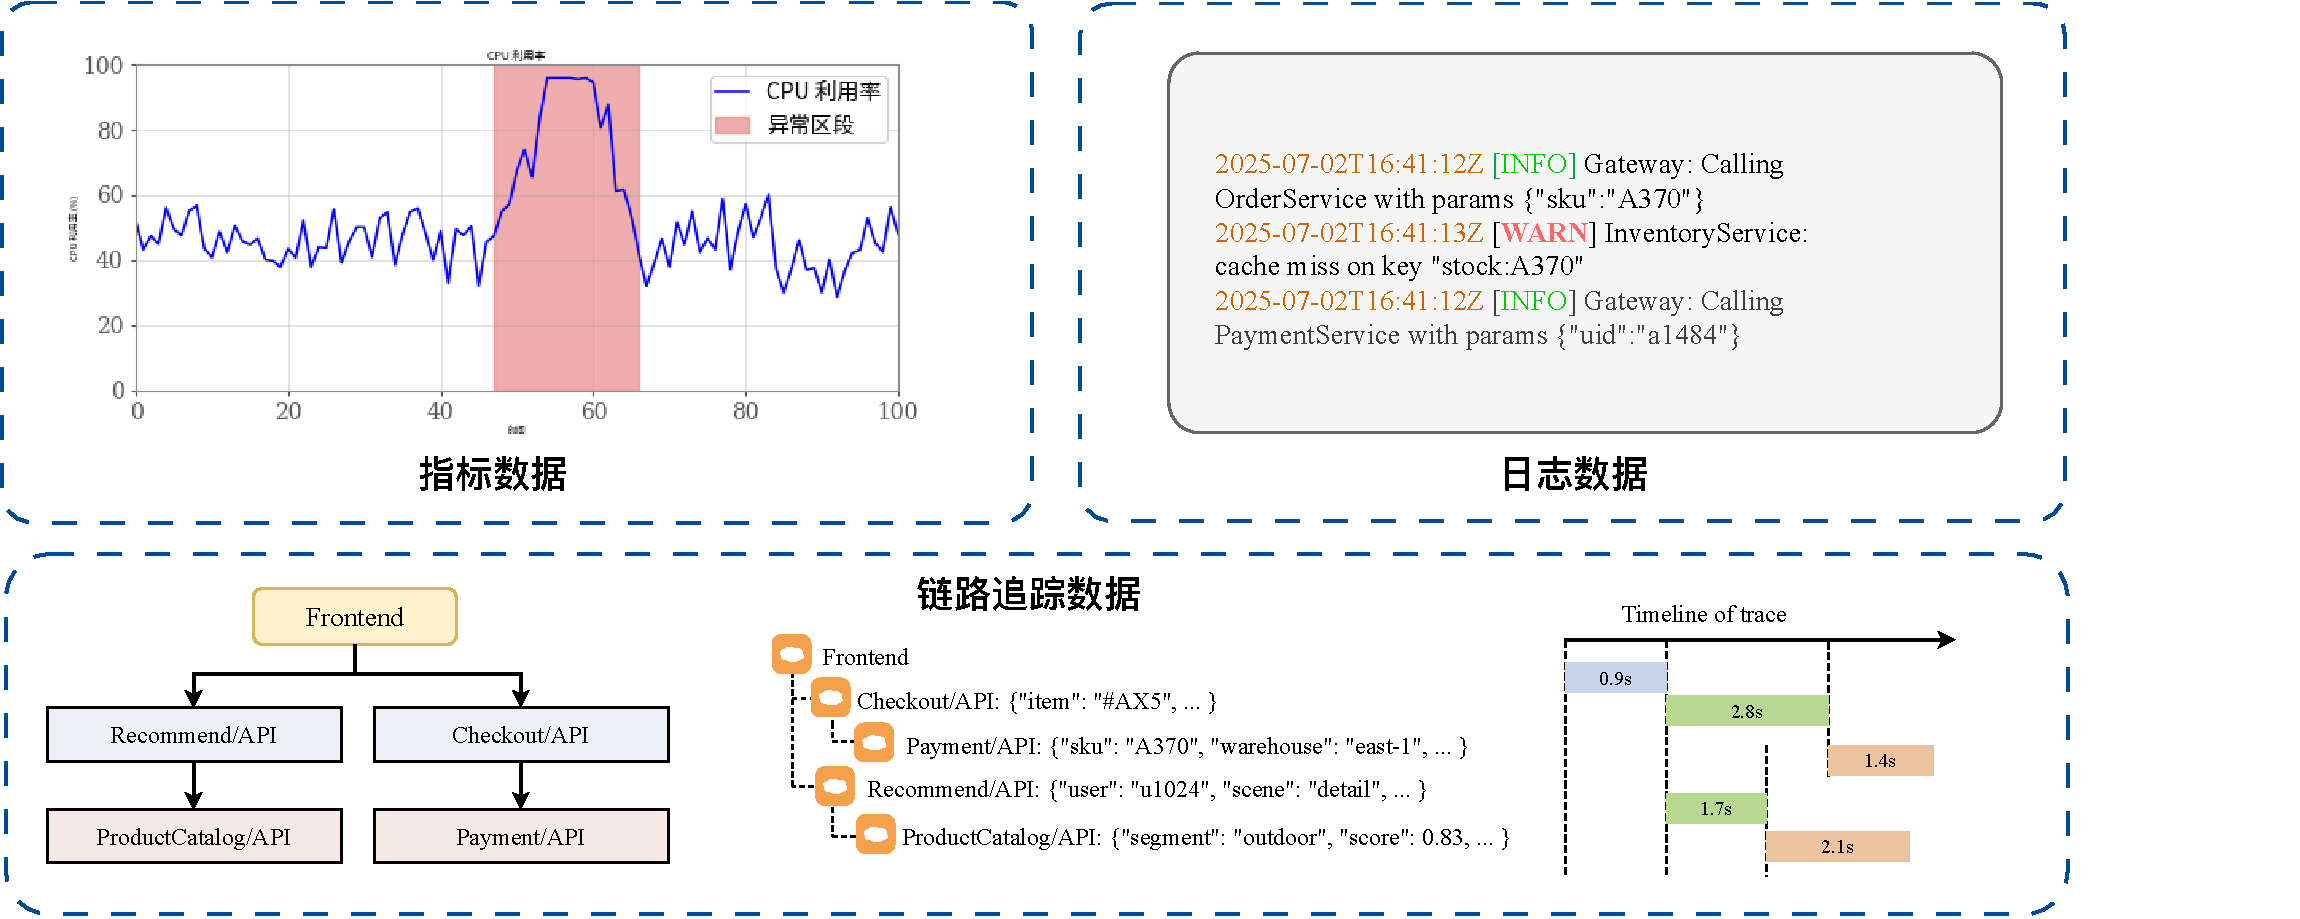
\includegraphics[width=\textwidth]{Figures-Src/Chap1-Introduction/multimodal-data/chart.pdf}
    \bicaption{\enspace 微服务故障诊断多模态数据示意}{\enspace Multimodal Data for Microservice Fault Diagnosis}
    \label{fig:multimodal-data}
\end{figure}

为持续感知系统运行状态，云服务系统通常围绕指标、日志和调用链路构建可观测性数据采集与分析体系\cite{sridharan2018distributed,opentelemetry2024,jia2020logdiagnosissurvey,huang2023tracepp}。由此形成的指标数据（Metrics）、日志数据（Logs）和调用链路数据（Traces）构成了微服务系统运行状态的三类基础观测信息。如图\ref{fig:multimodal-data}所示，以电商系统为例，这三类数据分别对应系统状态、异常语义和请求传播过程。指标数据通常以时间序列形式反映 CPU、内存、吞吐、错误率和时延等整体状态变化，适合描述服务和资源层面的运行波动；日志数据记录系统运行过程中的事件、异常栈和业务上下文，能够在故障发生时提供更细粒度的语义信息；调用链路数据则用于还原请求在多个服务之间的传播路径及其依赖关系。

在工程实践中，上述三类数据通常依托统一的可观测性工具链完成采集、传输、存储与分析。例如，OpenTelemetry\cite{opentelemetry2024}提供统一的遥测数据模型与采集接口，Prometheus\cite{prometheus2024}常用于指标采集与告警，Jaeger\cite{jaeger2024}用于分布式调用链路，Elasticsearch\cite{elasticsearch2024}等平台承担日志检索、聚合与分析任务。一次故障往往会在多个模态中留下相互关联的异常痕迹。若仅依赖单一类型的观测数据，通常难以完整把握故障的形成机制和传播过程。因此，面向多模态可观测数据的联合分析已成为微服务故障根因定位的重要前提。

微服务的异常告警仅表明系统已偏离正常运行状态，却无法直接回答故障源位于何处、异常如何沿依赖关系传播等关键问题。围绕这些问题展开的根因分析（Root Cause Analysis，RCA）是智能运维中的核心任务，其目标是在复杂运行现象与底层故障源之间建立可靠对应关系\cite{microservice-diagnosis-survey}。本文聚焦其中的根因定位问题，即在复杂运行现象中识别真实故障源及其传播链条。根因定位结果直接影响故障诊断效率、服务恢复时间以及后续运维决策的准确性，因此，根因定位始终是智能运维研究与工程实践中的关键环节。随着系统规模不断扩大，仅依赖运维人员根据指标、日志和调用链路数据进行人工排查，已难以满足复杂场景下对诊断速度、准确性和稳定性的要求\cite{microservice-diagnosis-survey,bao2023aiopsstandard}。

围绕根因分析，已有研究提出了多类诊断方法。早期工作主要依赖统计分析、规则匹配和依赖关系建模，对异常指标、日志模式和调用结构进行关联推断。随着监测数据规模增长和系统复杂度提升，图模型、机器学习和深度学习方法逐步被引入根因分析任务，用于从服务拓扑、调用依赖和历史故障实例中学习异常关联关系与根因判别模式\cite{microservice-diagnosis-survey}。这些方法提高了故障定位的自动化水平，但在异构数据利用、定位精度和结果可解释性方面仍有改进空间。

近年来，大语言模型（Large Language Model，LLM）在复杂语义理解和推理任务中的能力持续提升\cite{brown2020language,wei2022chain}。在此基础上，研究者开始探索将模型推理与外部工具调用结合起来，让模型在任务执行过程中主动获取额外信息并分步推进分析\cite{yao2022react,wang2024rcagent}。对于需要综合利用多源可观测数据的微服务故障根因定位任务，这类方法为大语言模型参与诊断分析提供了新的技术路径\cite{wang2024rcagent}。

%---------------------------------------------------------------------------%

\section{问题分析}

本节分析基于大语言模型的微服务故障根因定位所面临的关键问题。

近年来，大语言模型在复杂推理、任务规划、工具调用和多轮交互等方面表现出较强能力，已在代码生成、问答分析和智能体决策等任务中展现出良好的适应性\cite{yao2022react}。这一进展推动了大语言模型在运维智能体中的应用，也使其被逐步引入故障排查与根因定位任务。相较于传统依赖规则、统计特征或固定流程的方法，大语言模型能够处理自然语言描述，结合上下文组织分析过程，并根据当前信息动态调整后续动作，因此在复杂系统诊断中显示出较大潜力\cite{microservice-diagnosis-survey,wang2024rcagent}。

但大语言模型的推理能力并不等于稳定的根因定位能力。微服务系统中的故障并不会以根因本身直接暴露出来，运维人员和智能体首先观察到的通常只是请求超时、错误率升高、调用失败、实例负载波动等外部现象。由于服务之间存在复杂依赖关系，重试、熔断、限流、缓存和超时传播等机制又会持续改变异常的外在表现，同一根因在不同场景下可能呈现出不同症状，不同根因也可能表现出相似的异常现象。在这种情况下，智能体的根因定位并不是一次性给出结论，而是基于当前观测持续推理、不断调整检查对象与分析方向的动态过程。这一过程若过早停止，诊断往往只能停留在暴露的表象上，难以继续追溯真实的故障传播链条；若迟迟不能收敛，又容易在多处异常并发出现时不断引入新的分析方向，导致无效查询增多、上下文累积以及分析焦点漂移。因此，微服务场景中的故障根因定位需直面一个困难：在连续推理过程中既不能停在局部异常上，也不能在过多候选方向之间失去主线。


在故障诊断过程中，系统会逐步积累与根因定位相关的诊断依据、排查路径、分支条件和诊断结论，这些内容共同构成了诊断经验，并通常沉淀于 SOP、TSG、历史工单或者运维人员诊断记录之中。面对微服务场景下复杂且易扩散的异常现象，仅凭当前观测展开分析，智能体容易停留在局部异常上，或在多个候选方向之间不断调整。诊断经验能够为诊断过程提供可依赖的分析起点和路径参考，帮助智能体优先关注更可能指向根因的关键线索，并据此形成较为清晰的排查顺序。诊断经验的价值不仅在于保留历史结论，更在于保存故障场景与排查过程之间的对应关系，使智能体在面对复杂传播现象时能够借助既有诊断依据保持分析主线。

诊断经验要能在及时诊断中发挥作用，首先需要从历史故障场景中检索出与当前场景具有相似特征的案例，并将其诊断经验作为参考。要实现这一点，系统必须能够从多源观测中提炼出可与历史案例进行比较的故障特征。微服务故障通常通过指标、日志和调用链路等多类观测数据来刻画，三类数据分别记录状态变化、异常语义和请求传播路径，在结构形式、时间尺度和表达粒度上存在显著差异\cite{sridharan2018distributed,microservice-diagnosis-survey}。指标适合反映性能退化和资源失衡，日志能够提供更具体的异常上下文，调用链路则揭示请求在服务之间的传播关系，这些观测既相互补充，又在时间和拓扑两个维度上紧密耦合。某段调用时延升高，可能来自本地资源争用，也可能是下游故障向上游传播后的结果；某条错误日志究竟对应根因线索还是次生告警，也只有结合调用关系与时间才能判断。若无法将这些分散、异构且动态变化的观测数据组织为统一、可比较、可检索的故障表示，系统就难以准确比较当前故障与历史故障之间的相似性，也就难以检索出真正可供参考的诊断经验。

即使已经检索到相关诊断经验，这些经验也往往不能直接用于驱动智能体完成诊断。工程现场中的诊断经验虽然广泛存在于 SOP、TSG、历史工单和运维人员诊断记录中，但大多以半结构化文本的形式组织。此类文本能够保存历史故障的诊断过程和处理结论，却并不天然具备可执行性。通过传统检索或 RAG 方法召回之后，智能体虽然能够读取其中的内容，但很难稳定地将文本中的诊断描述转化为可持续执行的排查步骤。尤其是在涉及条件分支、路径切换和多步判断时，诸如“先检查某项指标，再结合日志判断；若满足某条件则转向下游服务，否则继续排查当前节点”这类文本表述，往往依赖隐含前提、上下文衔接和人工理解，难以被智能体直接遵循。

即使诊断经验已经被进一步整理为可供利用的诊断知识，在线根因定位仍然面临另一项困难，即历史诊断经验不可能覆盖全部故障场景。微服务系统持续演进，服务拓扑、部署环境和流量模式不断变化，新的异常组合会不断出现。若智能体严格依赖已有诊断经验，诊断过程容易在经验无法覆盖的位置停滞；若脱离已有诊断经验重新转向自由探索，前面提到的局部异常牵引、诊断范围扩张和分析主线丢失等问题又会再次出现。因此，在线根因定位还需要一种更稳定的执行方式，使智能体能够在诊断过程中判断当前路径是否仍值得继续、何时应跳出已有经验的限制并转向新的分析方向，同时控制排查范围，避免诊断过程过早中断或无序扩张。只有具备这样的能力，智能体才可能在真实环境中兼顾诊断效率与结果可靠性。


综上，基于大语言模型的微服务故障根因定位在实际落地过程中主要面临以下三个问题：

\begin{enumerate}[label=（\arabic*）]
    \item \textbf{多源异构观测难以统一表征。} 微服务故障分析依赖指标、日志和调用链路等多类观测数据，但不同类型数据在结构形式、时间尺度和表达粒度上差异明显，故障传播还会进一步拉大表面现象与真实故障源之间的距离。在缺乏统一表征框架的情况下，系统难以从复杂观测中提炼出可支持根因判断的稳定特征，也难以准确召回真正具有参考价值的历史诊断经验。

    \item \textbf{诊断经验难以知识化沉淀。} 现有 SOP、TSG、工单和专家经验大多以半结构化文本或静态流程的形式记录。这些信息虽然记录了历史诊断过程和处理结论，但在被检索召回后，智能体仍难以稳定把握其中的步骤顺序、条件分支和路径切换逻辑，因此，难以将其直接转化为可执行的诊断知识。

    \item \textbf{在线诊断过程难以在规范遵照与自主探索之间灵活协调。} 真实故障定位既不能机械套用已有诊断经验，也不能在缺乏依据时任由分析范围不断扩张。智能体需要根据当前诊断进展持续判断现有经验是否仍然适用、当前路径是否值得继续，以及何时转向新的分析方向。若缺乏这种切换能力，诊断过程就容易停滞在经验无法覆盖的位置，或在多个候选方向之间不断发散，从而影响根因定位的效率与可靠性。
    
\end{enumerate}

%---------------------------------------------------------------------------%
\section{研究工作}

针对上述问题，本文围绕故障表征、经验沉淀、在线诊断执行和系统实现四个方面展开研究，整体关系如图\ref{fig:research_work_overview}所示。围绕多模态观测条件下的微服务故障根因定位问题，本文依次回答三个核心问题：如何实现当前故障与历史故障的准确比较，如何将诊断经验沉淀为可执行的 SOP，以及如何在 SOP 引导下完成在线根因定位。与此对应，本文提出了故障指纹构建、SOP 自动化构建和 SOP 驱动在线诊断三项核心技术，并进一步实现了面向微服务故障根因定位的智能体平台。

\begin{figure}[htbp]
    \centering
    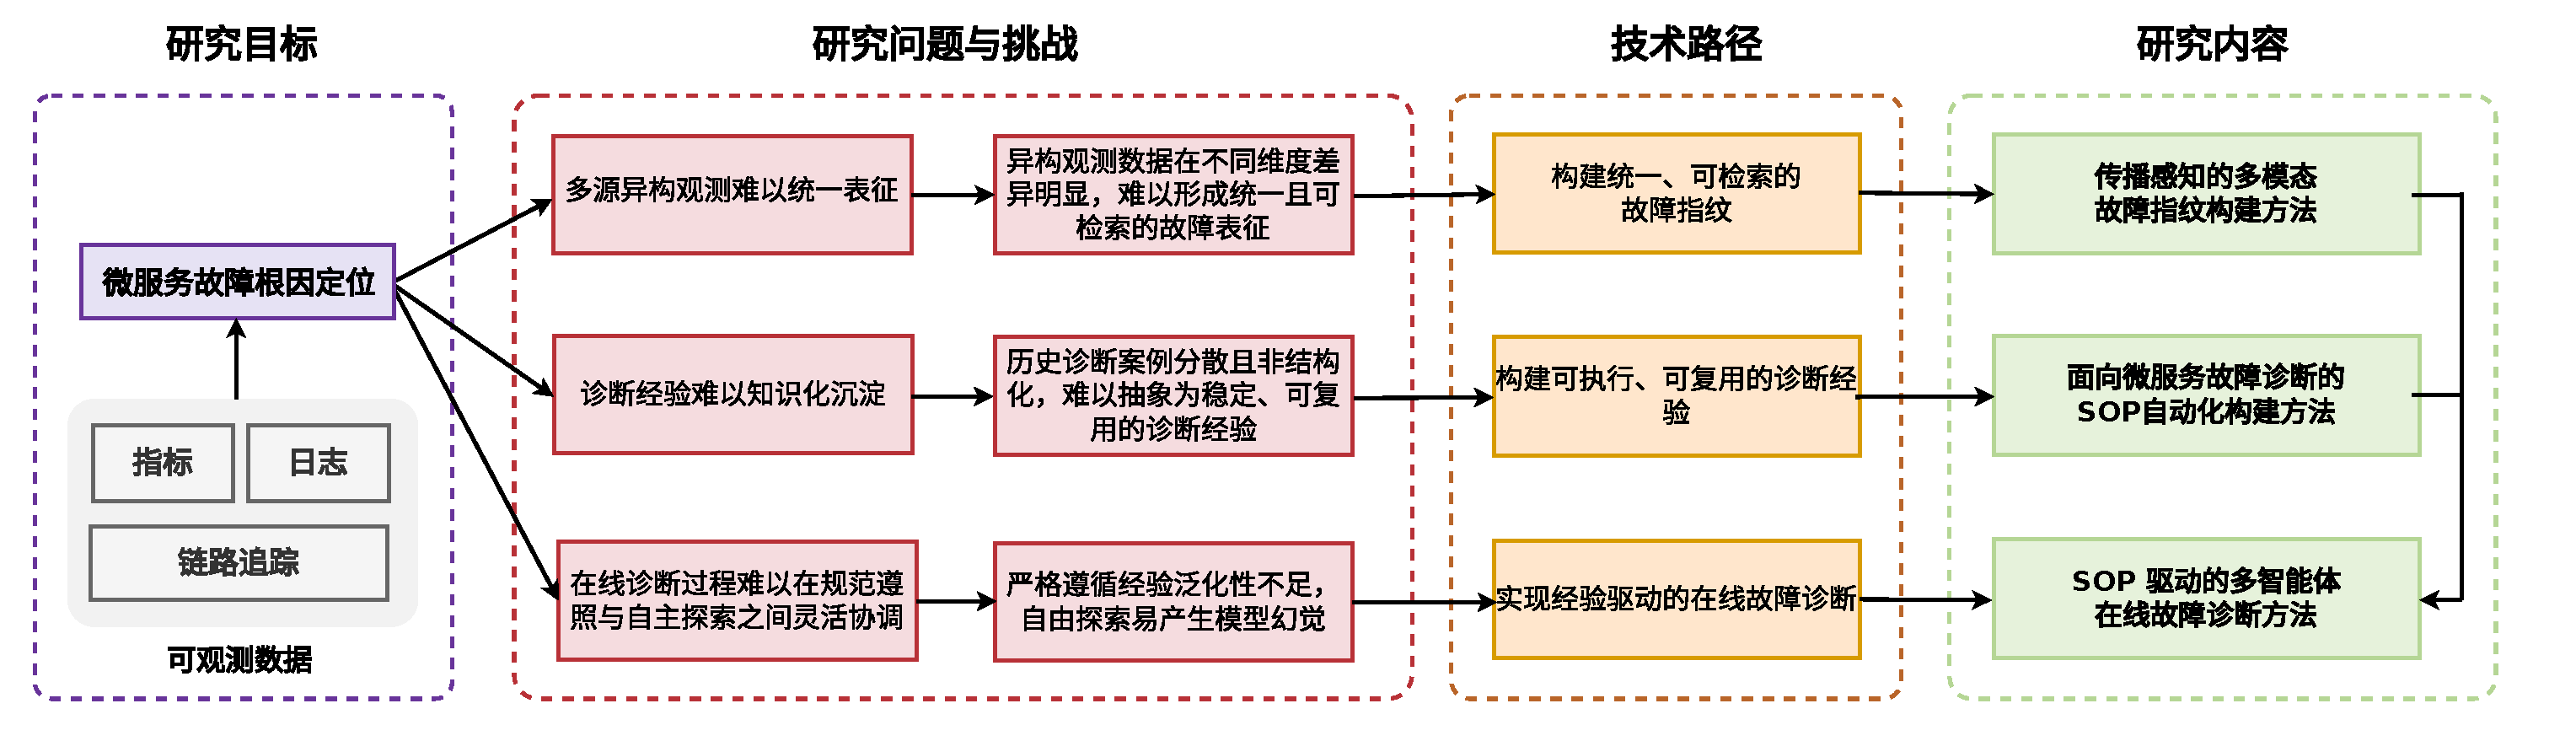
\includegraphics[width=\textwidth]{Figures-Src/Chap1-Introduction/research-work/chart.pdf}
    \bicaption{\enspace 本文研究工作的整体关系}{\enspace Overview of the Dissertation}
    \label{fig:research_work_overview}
\end{figure}

本文的主要工作如下：

（1）提出传播感知的多模态故障指纹构建方法。该方法从指标、日志和调用拓扑中提取指标形态、传播拓扑、时序关联、日志模式和跨模态耦合等特征，通过特征筛选生成可检索的故障指纹，为相似故障召回和 SOP 绑定提供基础。

（2）提出面向微服务故障诊断的 SOP 自动化构建方法。该方法采用三阶段流程实现从诊断经验到结构化知识的自动转化。首先，利用故障类型先验知识引导探索智能体生成较完整的 SOP执行轨迹；进而，通过语义归一化与权重计算，从多条执行轨迹中提取值得保留的决策单元；最后，由规则智能体将离散知识组织为可执行 SOP，实现诊断知识从具体场景向通用表达转化。

（3）提出 SOP 驱动的智能体在线故障诊断方法。该方法以诊断智能体为主要执行角色，遵循SOP进行推断，在焦点与感知域约束下协同观察智能体收集多模态证据；当既有 SOP 无法覆盖当前场景时，通过逃逸机制扩展新的诊断路径，并通过人工复核将诊断记录确认为新的故障实例并回流归档，用于故障指纹库与 SOP 知识库的增量更新。

（4）设计并实现故障诊断智能体平台。该平台同时支持离线知识构建与在线故障诊断两类任务，评估了故障指纹构建、SOP 自动化构建和 SOP 驱动在线诊断方法的工程可行性，并通过公开数据集实验验证了整体方案的有效性。

%---------------------------------------------------------------------------%
\section{论文组织}

论文后续内容安排如下。

第二章介绍微服务故障根因定位的相关技术与研究现状。该章先说明微服务故障根因定位的基础概念，包括微服务架构特点、故障分类及根因分析流程，再介绍大语言模型与智能体技术的基本思路，并梳理传统方法以及大语言模型的方法研究现状，最后总结现有工作的不足并引出本文的研究动机。

第三章介绍本文提出的诊断经验驱动微服务故障根因定位方法。该章首先给出方法总体框架，说明离线知识构建与在线故障诊断之间的关系；随后分别介绍故障指纹构建、SOP 自动化构建以及 SOP 驱动的在线诊断与知识更新方法；最后对本章内容进行小结。

第四章介绍故障诊断智能体平台的设计与实现。该章主要说明平台的总体架构、关键组成部分及其协同关系，并结合本文方法介绍平台如何支撑离线知识构建与在线故障诊断两类任务，最后对本章内容进行小结。

第五章为实验验证与分析。该章先给出研究问题，并介绍实验环境、数据集与评估指标，再分别开展故障指纹召回性能评估、SOP 构建有效性评估、端到端诊断性能评估和消融实验，最后对实验结果进行总结。

第六章为总结与展望。该章总结论文的主要贡献与创新点，并对后续研究工作进行展望，包括在更大规模系统中的应用前景以及与其他智能运维技术的结合方向。
